\documentclass[paper=a4, fontsize=11pt]{scrartcl}
%\usepackage{sectsty} % Allows for custom section title styling
\usepackage[T1]{fontenc}
\usepackage{fourier} % We're using the Utopia font because it's great.
\usepackage{enumerate} % Allows for custom enumeration types
\usepackage{tikz} % Graphics powered by TikZ!
\usepackage{xcolor} % More colors
\usepackage{listings} % For shell output
\usepackage{nameref} % Reference sections by name, since we're avoiding section numbering

\usetikzlibrary{positioning} % Relative positioning of nodes
\usetikzlibrary{automata} % Handy stuff for state machine diagrams

\tikzstyle{every state}=[fill=orange!30, draw=orange, very thick]
\tikzstyle{lock}=[->, draw=cyan, very thick, every to/.style={bend left=20}]
\tikzstyle{unlock}=[->, draw=magenta, very thick, every to/.style={bend left=20}]

\lstdefinestyle{ShellStyle} {
  basicstyle=\small\ttfamily,
  numbers=none,
  frame=tblr,
  columns=fullflexible,
  backgroundcolor=\color{blue!10},
  linewidth=0.9\linewidth,
  xleftmargin=0.1\linewidth
}

%\allsectionsfont{\centering \normalfont\scshape} % Center and semi-cap section titles
\newcommand{\horrule}[1]{\rule{\linewidth}{#1}} % Horizontal rule with weight arg

\title{
  \normalfont \normalsize 
  \textsc{New Mexico Tech} \\ [25pt]
  \horrule{0.5pt} \\[0.4cm]
  \huge CSE 325 --- Lab Project 4 \\ Thread Scheduler \\
  \horrule{2pt} \\[0.5cm]
}

\author{Rob Kelly \& Ian Neal \\ SANIC TEEM}
\date{\normalsize\today}

\begin{document}
\maketitle

%%% INTRODUCTION %%%
The SANIC TEEM Amazing Thread Scheduling Demonstration for Peace (hereafter referred to as \textit{the project}) is an interactive simulation of user-mode thread scheduling, designed to demonstrate two different thread scheduling policies:

\begin{description}
  \item[First Come, First Served] or \textit{FIFO}, wherein processes are scheduled to run in the order they arrive in the scheduling queue and will continue running until they either complete or block for I/O, and

  \item[Round Robin] or \textit{RR}, wherein processes are granted CPU time in discrete time slices or \textit{quanta}, after which they are moved to the end of the scheduling queue if they have yet to finish running.
\end{description}

Most of the codebase of this project was given as part of the lab assignment. We have implemented the functionality of the project in the following files:

\begin{itemize}
  \item Interface and implementation of scheduling-policy-independent functionality in \texttt{sched\_impl.h} and \texttt{sched\_impl.c}, respectively.

  \item Interface and implementation of \textit{FIFO}-scheduling functionality in \texttt{fifo\_impl.h} and \texttt{fifo\_impl.c}, respectively.

  \item Interface and implementation of \textit{RR}-scheduling functionality in \texttt{rr\_impl.h} and \texttt{rr\_impl.c}, respectively.

  \item Build targets for the added files and this README in the \texttt{Makefile}.
\end{itemize}

%%% BUILDING %%%
\section*{Building}
\begin{itemize}
  \item \texttt{make} to build the project normally.

  \item \texttt{make test} to run the provided testing harness.

  \item \texttt{make doc} to build this README. Requires \texttt{pdflatex} and a number of \LaTeX\hspace{0em} packages, all of which are included in the popular \textbf{TeX Live} distribution.

  \item \texttt{make clean} to clean up temporary files, build files, and output.
\end{itemize} 

%%% USAGE %%%
% Taken from scheduler.c:print_help()
\section*{Usage}
\texttt{./scheduler <sched\_impl> <queue\_size> <num\_threads> [iterations]}

\begin{itemize}
  \item \texttt{sched\_impl} may be \texttt{-fifo} to use \textit{FIFO} scheduling, \texttt{-rr} to use \textit{RR} scheduling, or \texttt{-dummy} to offload thread scheduling to the kernel.

  \item \texttt{queue\_size} is the number of threads that can be in the scheduler at one time.

  \item \texttt{num\_threads} is the number of worker threads to run.

  \item \texttt{iterations} is optionally the number of loops for each worker thread to run.
\end{itemize}


%%% EXAMPLES %%%
% Taken from the assignment PDF. We could replace this with our own program's output at some point.
\section*{Examples}
This first example uses \textit{FIFO} scheduling:
\begin{lstlisting}[style=ShellStyle]$
  $ ./scheduler -fifo 1 2 3
  Main: running 2 workers on 1 queue_size for 3 iterations
  Main: detaching worker thread 3075984304
  Main: detaching worker thread 3065494448
  Main: waiting for scheduler 3086474160
  Thread 3075984304: in scheduler queue
  Thread 3075984304: loop 0
  Thread 3075984304: loop 1
  Thread 3075984304: loop 2
  Thread 3075984304: exiting
  Thread 3065494448: in scheduler queue
  Thread 3065494448: loop 0
  Thread 3065494448: loop 1
  Thread 3065494448: loop 2
  Thread 3065494448: exiting
  Scheduler: done!
\end{lstlisting}
\pagebreak
Another example, this time using \textit{RR} scheduling:
\begin{lstlisting}[style=ShellStyle]$
  $ ./scheduler -rr 10 2 3
  Main: running 2 workers on 10 queue_size for 3 iterations
  Main: detaching worker thread 3075828656
  Main: detaching worker thread 3065338800
  Main: waiting for scheduler 3086318512
  Thread 3075828656: in scheduler queue
  Thread 3065338800: in scheduler queue
  Thread 3075828656: loop 0
  Thread 3065338800: loop 0
  Thread 3075828656: loop 1
  Thread 3065338800: loop 1
  Thread 3075828656: loop 2
  Thread 3065338800: loop 2
  Thread 3075828656: exiting
  Thread 3065338800: exiting
  Scheduler: done!
\end{lstlisting}

%%% DESIGN %%%
\section*{Design \& Implementation}
% Be sure and update this as we make progress...
\subsection*{Organization}
The execution of the project -- set-up, tear-down, and worker and scheduler routines -- is handled entirely by the framework established in the code given to us as part of the assignment. All of the functionality we've implemented is integrated modularly into the project by way of the function pointers contained in the \texttt{sched\_impl\_t} structures \texttt{sched\_fifo} and \texttt{sched\_rr} for the \textit{FIFO} and \textit{RR} scheduling policies, respectively. From a practical perspective, this is effectively an object-oriented schema, with \texttt{sched\_fifo} and \texttt{sched\_rr} inheriting from a more general implementation:

% TODO: diagram showing that thing what i just said

\subsection*{\textit{FIFO} Scheduling Policy}
% TODO

\subsection*{\textit{RR} Scheduling Policy}
% TODO

\subsection*{Scheduling Queue}
The scheduling queue is a simple FIFO queue implemented as a wrapper around a doubly-linked list, using the implementation provided in \texttt{list.h}. For both scheduling policies, the functionality of the queue itself is identical, as all policy-specific functionality has been offloaded to the worker-thread control system. The queue structure \texttt{sched\_queue}, typedeffed elsewhere as \texttt{sched\_queue\_t}, is implemented in \texttt{sched\_impl.c}, with all access methods passed as function pointers to the various scheduler implementations. These methods are all synchronized as described in \textbf{\nameref{design:sync}}, and are as follows:

\begin{itemize}
  \item \texttt{sched\_impl.c:init\_sched\_queue()} initializes and allocates space for an empty queue of a given size.
  \item \texttt{sched\_impl.c:destroy\_sched\_queue()} frees all resources used by the queue and any elements that may remain in the queue.
  \item \texttt{sched\_impl.c:enter\_sched\_queue()} inserts an element at the tail of the queue.
  \item \texttt{sched\_impl.c:leave\_sched\_queue()} removes a given element from the queue.
\end{itemize}

It should be noted that the elements of the queue are wrappers of type \texttt{list\_elem\_t}. The thread info items of type \texttt{thread\_info\_t} that are inserted into the queue keep track of their own wrappers as well as a pointer to the queue. This isn't an ideal design scheme, but is done to conform to the provided worker thread operation interface which passes only the thread info instance to queue methods.

\subsection*{Access Control \& Synchronization}
\label{design:sync}
Our implementation of access control to the scheduling queue uses a very similar strategy to the buffer access control strategy we implemented for Lab 3. We use two semaphores (referred to as the \textit{production} and \textit{consumption} locks) to synchronize the capacity of the queue, and one mutex access lock to enforce mutual exclusion of queue modification. When the queue is initialized, the production lock is initialized with a value the same as the capacity of the queue, and the consumption lock is initialized with a value of zero (locked). Insertion into the queue locks production and unlocks consumption, and vice-versa for removal of queue elements. The access lock is simply locked for critical sections where the queue is accessed for read/write operations. One new synchronization operation implemented here is the \texttt{wait\_for\_queue} operation, which blocks until there is an element in the queue; this is implemented by waiting for consumption to lock, then releasing the lock as soon as it is acquired. Figure~\ref{fig:qsync} shows the aforementioned capacity synchronization scheme, where semaphores are shown in orange, cyan edges denote the acquisition of a resource by a process, and magenta edges denote the unlocking of a resource by a process.

\begin{figure}[h]
  \centering
  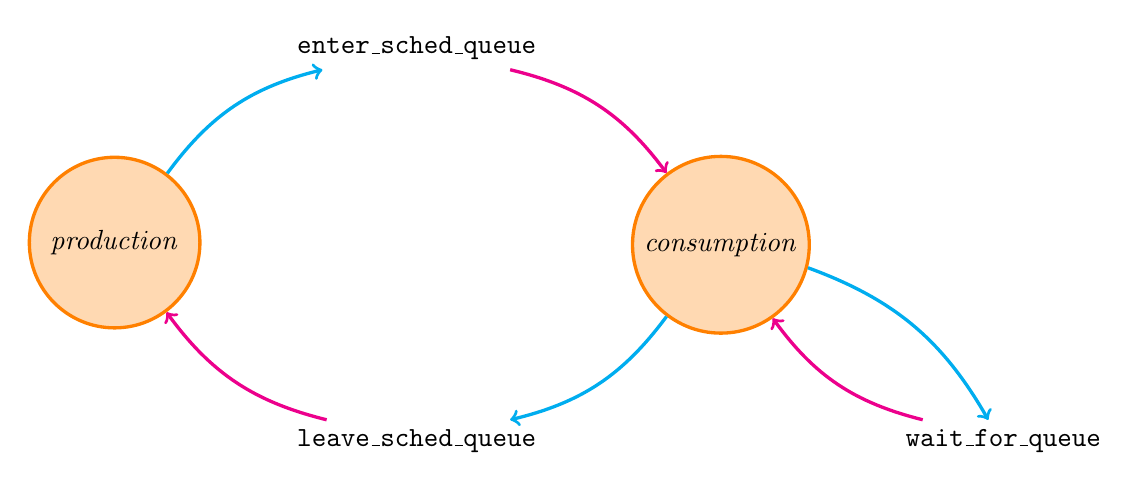
\begin{tikzpicture}[node distance = 2cm, auto]
    \node         (insert)                                     {\texttt{enter\_sched\_queue}};
    \node[state]  (production)  [below left = of insert]       {\phantom{-}\textit{production}\phantom{-}};
    \node[state]  (consumption) [below right = of insert]      {\textit{consumption}};
    \node         (remove)      [below left = of consumption]  {\texttt{leave\_sched\_queue}};
    \node         (wait)        [below right = of consumption] {\texttt{wait\_for\_queue}};

    \draw[lock]   (production)  to (insert);
    \draw[unlock] (insert)      to (consumption);
    \draw[lock]   (consumption) to (remove);
    \draw[unlock] (remove)      to (production);
    \draw[lock]   (consumption) to (wait);
    \draw[unlock] (wait)        to (consumption);
  \end{tikzpicture}
  \caption{Scheduling queue capacity synchronization.}
  \label{fig:qsync}
\end{figure}

%%% BUGS %%%
\section*{Known Bugs}
% TODO
None known.

\end{document}
